\documentclass[a4paper]{article}

\usepackage[spanish]{babel}
\usepackage{graphicx}
\usepackage{amsmath, amssymb}
\usepackage[margin=2cm]{geometry}
\usepackage{fancyhdr}
\usepackage{enumerate}
\usepackage[shortlabels]{enumitem}
\usepackage{parskip}
\usepackage[most]{tcolorbox}
\usepackage[hidelinks]{hyperref}
\usepackage{float}
\usepackage{booktabs}
\usepackage[hypcap=false]{caption}
\usepackage{mathrsfs}
\usepackage{tikz}
\setlength{\emergencystretch}{3em}


\lstset{
  language=Python,
  basicstyle=\ttfamily\small,
  keywordstyle=\color{blue!70!black}\bfseries,
  commentstyle=\color{gray}\itshape,
  stringstyle=\color{red!60!black},
  showstringspaces=false,
  breaklines=true,
  frame=single,
  framerule=0.4pt,
  numbers=left,
  numbersep=8pt,
  numberstyle=\tiny\color{gray},
  xleftmargin=15pt
}


% cabecera
\pagestyle{fancy}
\fancyhead[l]{Astroestadística}
\fancyhead[c]{Parcial 3}
\fancyhead[r]{\today}
\fancyfoot[c]{\thepage}
\renewcommand{\headrulewidth}{0.2pt} % linea horizontal


\begin{document}


\section{Problema}

\textbf{Modelo de estrellas variables.} Se adjunta el archivo \texttt{mw\_cepheids.csv}, que contiene observaciones de un conjunto de estrellas Cefeidas (Breuval+, 2021). Para cada estrella se reportan su período de pulsación (en días), paralaje (en mas) y sus magnitudes en las bandas V e I. La relación período--luminosidad de las Cefeidas puede modelarse mediante la ecuación

$$
M_i = a + b \log_{10}(P_i) + \varepsilon_i,
$$

donde $M$ es la magnitud absoluta, $P$ el período y los errores observacionales son independientes y siguen una distribución normal $\varepsilon_i \sim N(0, \sigma^2)$. Suponga que la desviación estándar de los errores es conocida e igual a $\sigma = 0.3$ mag.

Para los parámetros del modelo considere distribuciones a priori normales e independientes entre sí, ambas con $\mu = 0$ y $\sigma^2 = 10^2$.


\subsection{Inspección inicial de los datos}

Antes de comenzar con los incisos, se cargó el archivo de datos en Python y se revisaron sus primeras filas:

\begin{verbatim}
df = pd.read_csv('mw_cepheids.csv')
print(df.head())
\end{verbatim}

El resultado obtenido fue:

\begin{verbatim}
        _RAJ2000     _DEJ2000     Per     plx    Vmag    Imag
0            deg          deg       d     mas     mag     mag
1    -----------  -----------  ------  ------  ------  ------
2    916.456.086  +26.3292228  11.302     311   9.735     NaN
3  1.052.492.503  -87.089.917   8.014     383  10.100   8.708
4  1.007.812.989  +20.9391108   3.788     370     NaN     NaN
\end{verbatim}

\subsection{Parte A}

\begin{enumerate}[a)]
    \item Lea el archivo \texttt{mw\_cepheids.csv} y realice un gráfico de dispersión de la magnitud absoluta $M$ en función de $\log_{10}(P)$. Describa brevemente la tendencia observada.
    
\begin{lstlisting}
plx_arcsec = df['plx'].values / 1000                         # paralaje [arcsec]
x  = np.log10(df['Per'].values)                           # log10(P_i) [adim]
y  = df['Vmag'].values + 5*np.log10(plx_arcsec) + 5        # M_i [mag]
n  = len(x)
sigma = 0.3                                                # desv. est. conocida
\end{lstlisting}

    \begin{center}
        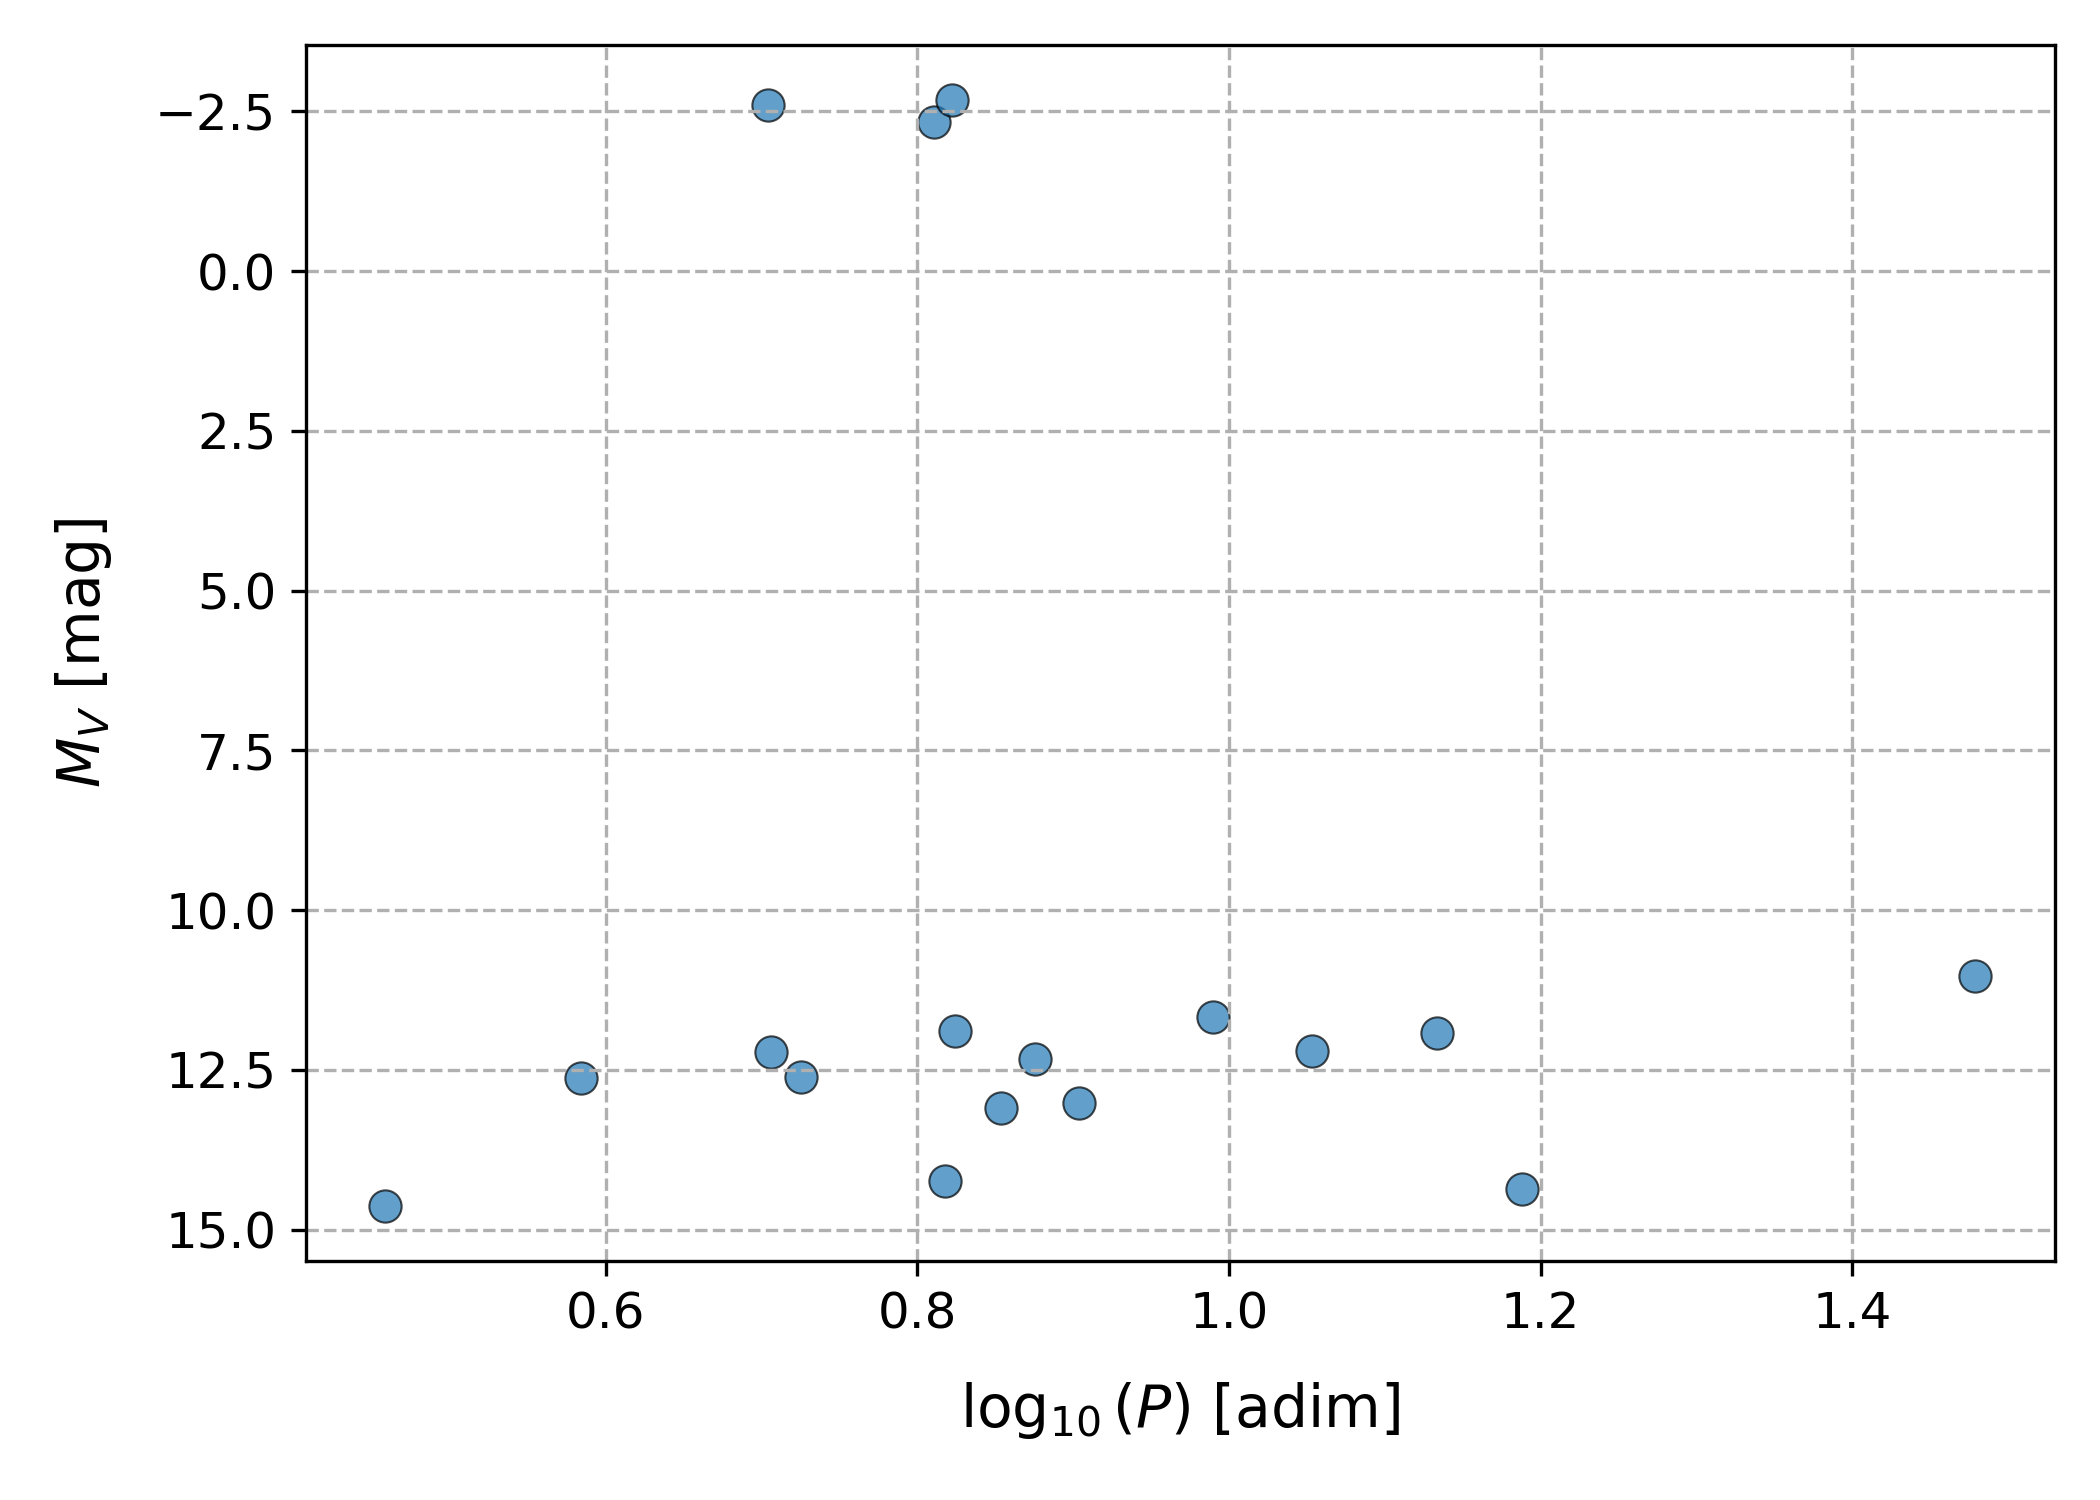
\includegraphics[width=0.82\textwidth]{dispersion.png}
        \captionof{figure}{Gráfico de dispersión de la magnitud absoluta en la banda V ($M_V$) en función del logaritmo del período ($\log_{10}(P)$) para la muestra seleccionada del dataset.}
    \end{center}
    
    \item Escriba la función de verosimilitud para los parámetros $a$ y $b$.
    
    Como $y_i\mid M(a,b)\sim\mathcal{N}(a+bx_i,\,\sigma^2)$ de forma
independiente para cada observación, la verosimilitud conjunta es
$L(y\mid M(a,b))=\prod_i f(y_i\mid M(a,b))$. Descartando la constante
de normalización:
\begin{equation}
  L\!\left(y\mid M(a,b)\right)
  \;\propto\;
  \exp\!\left(-\frac{1}{2\sigma^2}\sum_{i=1}^{n}
              \bigl(y_i - a - bx_i\bigr)^2\right).
  \label{eq:vero}
\end{equation}

    
    \item Escriba la distribución posterior conjunta de $a$ y $b$, ignorando constantes de normalización.
    
    Por el teorema de Bayes, $P(M(a,b)\mid y)\propto
L(y\mid M(a,b))\cdot f(a,b)$, con prior
$f(a,b)\propto\exp\!\bigl(-\tfrac{a^2+b^2}{200}\bigr)$:
\begin{equation}
  P\!\left(M(a,b)\mid y\right)
  \;\propto\;
  \exp\!\left(
    -\frac{1}{2\sigma^2}\sum_{i}(y_i-a-bx_i)^2
    -\frac{a^2+b^2}{200}
  \right).
  \label{eq:post}
\end{equation}

    \item Encuentre los valores de máxima probabilidad a posteriori (MAP) de $a$ y $b$.
    
    Se toma el logaritmo de~\eqref{eq:post} y se igualan a cero las
derivadas parciales respecto de $a$ y $b$.
Las ecuaciones resultantes son \textbf{lineales} en $(\hat{a},\hat{b})$
y forman el sistema $\mathbf{M}\vec\theta = \vec Z$:
\begin{equation}
  \underbrace{\begin{bmatrix}
    n + \dfrac{\sigma^2}{100} & \displaystyle\sum_i x_i \\[8pt]
    \displaystyle\sum_i x_i   & \displaystyle\sum_i x_i^2
                                +\dfrac{\sigma^2}{100}
  \end{bmatrix}}_{\mathbf{M}}
  \underbrace{\begin{bmatrix}\hat{a}\\\hat{b}\end{bmatrix}}_{\vec\theta}
  =
  \underbrace{\begin{bmatrix}
    \displaystyle\sum_i y_i \\[4pt]
    \displaystyle\sum_i x_iy_i
  \end{bmatrix}}_{\vec Z}.
  \label{eq:sistema}
\end{equation}

Los términos $\sigma^2/100$ en la diagonal provienen de derivar el
término de la previa $-\tfrac{a^2+b^2}{200}$.

\begin{lstlisting}
sum_x  = x.sum();    sum_x2 = (x**2).sum()   # estadisticos
sum_y  = y.sum();    sum_xy = (x*y).sum()

M_mat = np.array([[n + sigma**2/100, sum_x ],
                   [sum_x,           sum_x2 + sigma**2/100]])  # matriz M
Z_vec = np.array([sum_y, sum_xy])                              # vector Z

a_map, b_map = np.linalg.solve(M_mat, Z_vec)   # resuelve M theta = Z
\end{lstlisting}

La solución numérica obtenida para los estimadores MAP fue:
\begin{equation}
  \boxed{\hat a = 7.2506, \qquad \hat b = 3.1462.}
  \label{eq:map-numerico}
\end{equation}
Es decir, el modelo ajustado con los valores de máxima probabilidad a posteriori queda
\begin{equation}
  \widehat{M}_{\text{MAP}} = 7.2506 + 3.1462\,\log_{10}(P).
\end{equation}

    \item Demuestre que la distribución posterior conjunta de $(a, b)$ es una normal bivariada y determine su media y matriz de covarianza.
    
    Se expande el cuadrado en~\eqref{eq:post}:
\[
  \sum_i(y_i-a-bx_i)^2
  = na^2 + 2ab\!\sum_i x_i + b^2\!\sum_i x_i^2
    - 2a\!\sum_i y_i - 2b\!\sum_i x_iy_i
    + \underbrace{\sum_i y_i^2}_{\text{cte en }(a,b)}.
\]
Sustituyendo en~\eqref{eq:post} y agrupando con el término de la previa,
el exponente toma la forma cuadrática:
\begin{equation}
  \ln P(M(a,b)\mid y)
  = -\frac{1}{2}\!\left(Aa^2 + 2Bab + Cb^2 - 2Da - 2Eb\right)
    + \mathrm{cte},
  \label{eq:forma-cuad}
\end{equation}
con coeficientes
\begin{align}
  A &= \frac{n}{\sigma^2}+\frac{1}{100}, &
  B &= \frac{\sum_i x_i}{\sigma^2}, &
  C &= \frac{\sum_i x_i^2}{\sigma^2}+\frac{1}{100},
  \label{eq:ABC}\\
  D &= \frac{\sum_i y_i}{\sigma^2}, &
  E &= \frac{\sum_i x_iy_i}{\sigma^2}.&&
  \label{eq:DE}
\end{align}

La expresión~\eqref{eq:forma-cuad} es exactamente el núcleo de una
distribución normal bivariada.  
Por tanto:
\begin{equation}
  (a,b)\mid y \;\sim\; \mathcal{N}_2\!\bigl((\hat{a},\hat{b}),\,\Sigma\bigr),
  \label{eq:posterior-normal}
\end{equation}
donde $(\hat{a},\hat{b})$ es la solución de~\eqref{eq:sistema} (media
$=$ moda para una normal), la \textbf{matriz de precisión} es
\begin{equation}
  \Sigma^{-1}
  = \begin{bmatrix}A & B \\ B & C\end{bmatrix},
  \qquad
  \Sigma
  = \frac{1}{AC-B^2}\begin{bmatrix}C&-B\\-B&A\end{bmatrix}.
  \label{eq:cov}
\end{equation}

\begin{lstlisting}
A = n/sigma**2 + 1/100
B = sum_x/sigma**2
C = sum_x2/sigma**2 + 1/100

Prec  = np.array([[A, B], [B, C]])  # matriz de precision 
Sigma = np.linalg.inv(Prec)         # covarianza posterior
\end{lstlisting}

La solución numérica obtenida para estas matrices fue:
\begin{equation}
  \Sigma^{-1}=
  \begin{bmatrix}
    188.8989 & 165.8626\\
    165.8626 & 155.9583
  \end{bmatrix}
  \label{eq:precision-numerica}
\end{equation}
\begin{equation}
  \Sigma=
  \begin{bmatrix}
    0.0800 & -0.0851\\
    -0.0851 & 0.0969
  \end{bmatrix}
  \label{eq:covarianza-numerica}
\end{equation}
Así, la posterior conjunta queda completamente determinada por la media MAP de~\eqref{eq:map-numerico} y la matriz de covarianza posterior de~\eqref{eq:covarianza-numerica}.

    
    \item Utilice el resultado anterior para generar $10^4$ muestras aleatorias de la distribución posterior conjunta de $(a, b).$
    
    Se usa el resultado~\eqref{eq:posterior-normal}:
\begin{lstlisting}
np.random.seed(42)
theta_s = np.random.multivariate_normal([a_map, b_map], Sigma, size=int(10e4))
a_s, b_s = theta_s[:, 0], theta_s[:, 1]   # muestras marginales de a y b
\end{lstlisting}

    
    \item A partir de las muestras simuladas, estime un intervalo de credibilidad del 95\% para $a$ y $b$.
    
    Se obtienen como los percentiles 2.5 y 97.5 de las muestras:
\begin{lstlisting}
ci_a = np.percentile(a_s, [2.5, 97.5])   # IC 95% para a
ci_b = np.percentile(b_s, [2.5, 97.5])   # IC 95% para b
\end{lstlisting}

    
    \item Utilice las muestras posteriores para estimar la distribución posterior de la magnitud absoluta de una Cefeida con período $P = 12$ días. Reporte la media posterior y un intervalo de credibilidad del 95\% para la magnitud absoluta predicha.
    
    Para cada muestra $(\tilde{a},\tilde{b})$ de la posterior se predice
$\tilde{M} = \tilde{a} + \tilde{b}\log_{10}(12)$ la colección de
$\tilde{M}$ aproxima la distribución posterior de la magnitud absoluta:
\begin{lstlisting}
x_new  = np.log10(12)                          # log10(P) para P = 12 dias
M_pred = a_s + b_s * x_new                    # distribucion predictiva posterior
mu_pred, ci_pred = M_pred.mean(), np.percentile(M_pred, [2.5, 97.5])
\end{lstlisting}

    
    \item Grafique la relación período--luminosidad utilizando la recta correspondiente a los valores MAP de los parámetros. Sobre el mismo gráfico, incluya una banda de credibilidad del 95\% obtenida a partir de las simulaciones de la distribución posterior.
    
    Se evalúa cada muestra $(\tilde{a},\tilde{b})$ en una grilla de
$\log_{10}(P)$ y se toman los percentiles 2.5 y 97.5 columna a columna:

\begin{lstlisting}
x_grid = np.linspace(x.min(), x.max(), 300)
M_grid = a_s[:, None] + b_s[:, None]*x_grid  # (10000, 300): curva por muestra
lo, hi = np.percentile(M_grid, [2.5, 97.5], axis=0)
\end{lstlisting}

\begin{center}
    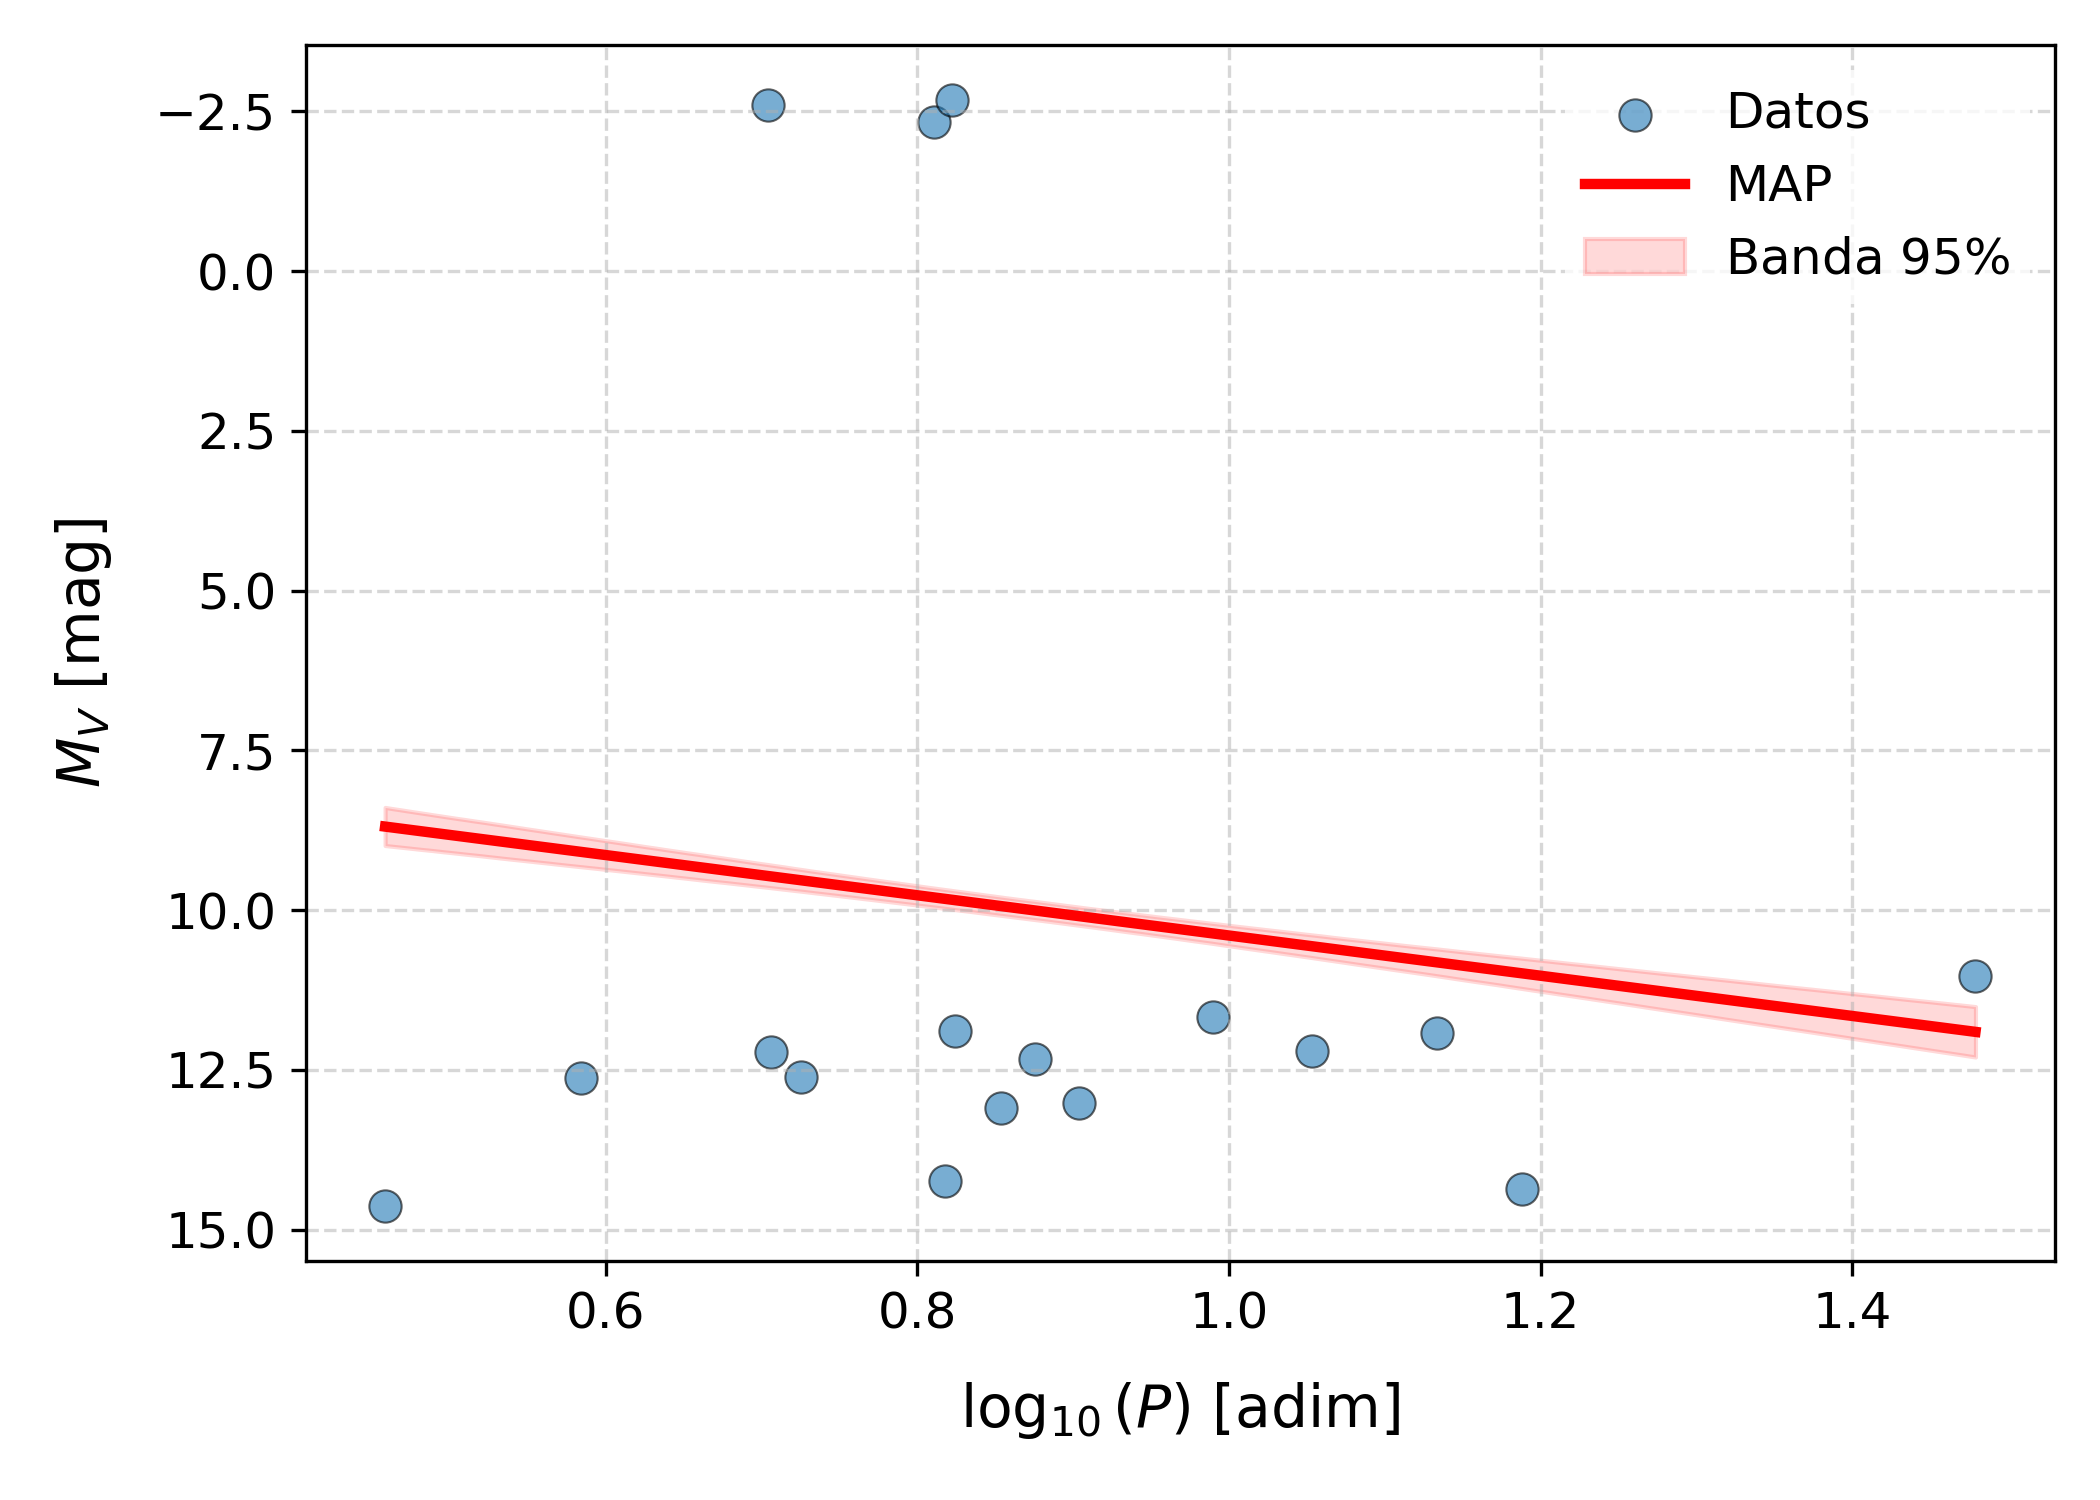
\includegraphics[width=0.82\textwidth]{pl_band.png}
    \captionof{figure}{Relación período--luminosidad ajustada con la recta MAP y banda de credibilidad posterior del 95\%.}
\end{center}

    
    \item Compare los resultados obtenidos mediante el enfoque bayesiano con los que se obtendrían usando una regresión lineal clásica por mínimos cuadrados. Discuta semejanzas y diferencias entre ambos enfoques.
    
    Para la regresión lineal clásica por mínimos cuadrados se usó:
\begin{lstlisting}
X_mat = np.column_stack([np.ones(n), x])
a_ols, b_ols = np.linalg.lstsq(X_mat, y, rcond=None)[0]
\end{lstlisting}

El resultado numérico fue:
\begin{equation}
  \hat a_{\text{OLS}} = 7.2538, \qquad
  \hat b_{\text{OLS}} = 3.1431
\end{equation}

Estos valores son muy cercanos a los estimadores MAP de~\eqref{eq:map-numerico},
porque la prior normal usada es amplia y el término de regularización
$\sigma^2/100=0.0009$ es pequeño. La diferencia principal es de
interpretación: el enfoque bayesiano entrega una distribución posterior
para $(a,b)$ y permite construir intervalos de credibilidad, mientras que
OLS entrega estimadores puntuales e intervalos de confianza frecuentistas.
Además, con las muestras posteriores la incertidumbre se propaga de forma
directa a nuevas predicciones.
\end{enumerate}

\subsection{Parte B}

\begin{enumerate}[a)]
	\item Obtenga intervalos de confianza bootstrap del $95\%$ para los parámetros $a$ y $b$. Compare estos resultados con los intervalos de credibilidad bayesianos.
	\item Genere $10^4$ conjuntos de datos sintéticos a partir del modelo posterior predictivo y compare la distribución de residuos simulados con la observada mediante una prueba de Kolmogorov-Smirnov.
	\item Considere un modelo alternativo
	$$
	M = a+b\log_{10}(P) + c[\log_{10}(P)]^2
	$$
	Obtenga los valores MAP de los parámetros y compare el poder predictivo de este modelo con el modelo lineal utilizando remuestreo bootstrap.
\end{enumerate}

\end{document}
